%%%%%%%%%%%%%%%%%%%%%%%%%%%%%%%%%%%%%%%%%
% a0poster Portrait Poster
% LaTeX Template
% Version 1.0 (22/06/13)
%
% The a0poster class was created by:
% Gerlinde Kettl and Matthias Weiser (tex@kettl.de)
% 
% This template has been downloaded from:
% http://www.LaTeXTemplates.com
%
% License:
% CC BY-NC-SA 3.0 (http://creativecommons.org/licenses/by-nc-sa/3.0/)
%
%%%%%%%%%%%%%%%%%%%%%%%%%%%%%%%%%%%%%%%%%

%----------------------------------------------------------------------------------------
%	PACKAGES AND OTHER DOCUMENT CONFIGURATIONS
%----------------------------------------------------------------------------------------

\documentclass[a0,portrait]{a0poster}
\usepackage[nomath]{lmodern}


\usepackage{multicol} % This is so we can have multiple columns of text side-by-side
\columnsep=100pt % This is the amount of white space between the columns in the poster
\columnseprule=3pt % This is the thickness of the black line between the columns in the poster

\usepackage[svgnames]{xcolor} % Specify colors by their 'svgnames', for a full list of all colors available see here: http://www.latextemplates.com/svgnames-colors

\usepackage{times} % Use the times font
%\usepackage{palatino} % Uncomment to use the Palatino font

\usepackage{graphicx} % Required for including images
\graphicspath{{figures/}} % Location of the graphics files
\usepackage{booktabs} % Top and bottom rules for table
\usepackage[font=small,labelfont=bf]{caption} % Required for specifying captions to tables and figures
\usepackage{amsfonts, amsmath, amsthm, amssymb} % For math fonts, symbols and environments
\usepackage{wrapfig} % Allows wrapping text around tables and figures
\usepackage{color}
\usepackage{colortbl}
%\def\beamer@loadlater{\usecolortheme[rgb={0.2,0.2,0.7}]{structure}}}
\definecolor{structurecol}{RGB}{51,51,178}
\newcommand{\structure}[1]{{\color{structurecol}#1}}
%\newcommand{\structure}[1]{{\color{NavyBlue}#1}}

% Math commands
\newcommand{\sys}{S}
\newcommand{\diss}{d}
\newcommand{\learn}{\mathcal{A}}
\newcommand{\free}{\mathcal{M}}
\newcommand{\D}{\mathcal{D}}
\newcommand{\R}{\mathbb{R}}
\newcommand{\nsamp}{N}
\newcommand{\norm}[1]{\left\lVert#1\right\rVert}

\begin{document}

%----------------------------------------------------------------------------------------
%	POSTER HEADER 
%----------------------------------------------------------------------------------------

% The header is divided into two boxes:
% The first is 75% wide and houses the title, subtitle, names, university/organization and contact information
% The second is 25% wide and houses a logo for your university/organization or a photo of you
% The widths of these boxes can be easily edited to accommodate your content as you see fit

\begin{minipage}[ht!]{\linewidth}
  \includegraphics[width=\linewidth]{poster_top.png}
\end{minipage}

\vspace{2.0cm}

\begin{center}
\textbf{\bf\huge\color{structurecol}In-context learning for model-free system identification\\[1.0cm]}
\large M.~Forgione, F.~Pura, and D.~Piga\\[0.3cm]
\normalsize IDSIA Dalle Molle Insitute for Artificial Intelligence \\[0.3cm]
%$^2$Depto de Física, FFCLRP/USP\\[0.2cm]
\small{\tt \{marco.forgione, filippo.pura, dario.piga\}@idsia.ch}
\end{center}

\vspace{1cm} % A bit of extra whitespace between the header and poster content
\begin{center}
\large \textbf{\structure{Meta-learning of dynamical systems}} \\[0.3cm]
\end{center}
{In standard identification, we improve as we see more data from a \structure{single system}. Can we also learn from similar ones?}
\begin{itemize}
% \item  \structure{Collection} of datasets $\D^{(i)} = (u_{1:\nsamp}^{(i)}, y_{1:\nsamp}^{(i)}), i=1,2,\dots$ from 
%\structure{random dynamical systems}  $\sys^{(i)}$ fed by random input $u_{1:\nsamp}^{(i)}$
 \item  \structure{Collection} of datasets $\D^{(i)} = (u_{1:\nsamp}^{(i)}, y_{1:\nsamp}^{(i)})$ from different, but \structure{related dynamical systems}  $\sys^{(i)}$ available
 %fed by random input $u_{1:\nsamp}^{(i)}$

 \item Can we get better at identifying $\sys^{(i)}$ as we observe more datasets $\D^{(j)}$? 
 Can we \structure{learn to learn} dynamical systems?
\end{itemize}
\vskip 1em
\begin{center}
\large \textbf{\structure{In-context learning approach}} \\[0.3cm]
\end{center}

\begin{itemize}
\item \structure{Transformers} are expressive  as \structure{a programming language}. We can train them to \structure{behave like algorithms}
\item We provide them with a \structure{context} of input/output data and a \structure{task}.
 They must \structure{learn to identify} systems to solve the task
\item If we manage to train the Transformer over \structure{a class} of dynamical systems, it becomes
a \structure{meta model} of that class!
\end{itemize}
\noindent
%\vskip 2em

\begin{multicols}{2}
%% One-step prediction
\begin{center}
{\large \textbf{\structure{One-step prediction}}} \\
\vskip -1.5cm
{\small $$\hat y_{k+1} = \free_\phi(u_{1:k}, y_{1:k})$$}
\vskip 1.5em
\includegraphics[height=17cm]{figures/architecture/decoder_architecture.png}
%\vspace{5cm}
\vspace{4cm}\\
%\vspace{2cm}\\
Linear system class\\
\includegraphics[height=9cm]{figures/lin_one_step_batch_single.png}\\
Wiener-Hammerstein system class\\
\includegraphics[height=9cm]{figures/wh_one_step_batch_single.png}
\end{center}%\vspace{1cm}

%% Multi-step simulation
\begin{center}
{\large \textbf{\structure{Multi-step simulation}}} \\
\vskip -1.5cm
{\small $$\hat y_{m+1:N} = \free_\phi(u_{1:m}, y_{1:m}, u_{m+1:N})$$}
\vskip .5em
\includegraphics[height=21cm]{figures/architecture/encoder_decoder_architecture.png}

\vspace{2cm}
Linear system class\\
\includegraphics[height=9cm]{figures/lin_sim_batch_single.png}\\
Wiener-Hammerstein system class\\
\includegraphics[height=9cm]{figures/wh_sim_batch_single.png}\\
\end{center}
\end{multicols}

%\vskip 2cm
\begin{center}
{\large \textbf{\structure{Future works}} \\[0.3cm]}
\end{center}
%Several open research directions including:
\begin{itemize}
\item \structure{Transfer learning}  from a system class to another one and \structure{fine tuning} to a specific system instance
\item \structure{Curriculum learning} to solve complex tasks starting from models learned on simpler ones%for learning of complex system classes/tasks starting from simpler ones
\item Analysis of the effect of \structure{noise} during meta training. Can it help generalization?
Does it hinder optimization? 
\end{itemize}


\end{document}